%dvipsnames are for the xcolor package to include colors like RubineRed
\documentclass[dvipsnames,table,aspectratio=169]{beamer}
\usepackage{scalerel}
\usepackage{pgfplots}
\usepackage{xcolor}
\usepackage{graphicx}
\usepackage{animate}
\usepackage{xlop}
\usepackage{tikz}
\usepackage{listings}
\usepackage[ruled]{algorithm2e}
\usepackage{float}
\usepackage[normalem]{ulem} % sout
\usepackage{bm} % bold plus in math
\usepackage{tabu}
\usepackage{fancyvrb}
\usepackage{amsmath,amssymb,amsfonts}
\usepackage{booktabs}
\usepackage{enumitem}
\usepackage{multirow}
\usetikzlibrary{shadows,shapes,calc,snakes,positioning,plotmarks}
\tikzset{onslide/.code args={<#1>#2}{%
  \only<#1>{\pgfkeysalso{#2}} % \pgfkeysalso doesn't change the path
}}

\tikzset{temporal/.code args={<#1>#2#3#4}{%
  \temporal<#1>{\pgfkeysalso{#2}}{\pgfkeysalso{#3}}{\pgfkeysalso{#4}} % \pgfkeysalso doesn't change the path
}}


\usepackage{minted}
\usemintedstyle{default}

\definecolor{darkgreen}{rgb}{0.0,0.2,0.13}
\newcommand{\cf}{\texttt{CF}}
\newcommand{\fadd}{\textsc{Add}\xspace}
\newcommand{\fmul}{\textsc{Mul}\xspace}
%comments in algorithm code
\newcommand\mycommfont[1]{\footnotesize\ttfamily\textcolor{blue}{#1}}
\SetCommentSty{mycommfont}
\newcommand{\colA}{blue} % A1
\newcommand{\colB}{red} % M1
\newcommand{\colC}{darkgreen} %M2
\newcommand{\colD}{orange} %A3
\newcommand{\colE}{violet} %A2
\newcommand{\colF}{cyan} %A4
\newcommand{\colG}{olive} %A5
\newcommand{\instr}[1]{\texttt{#1}}

\newcommand{\assembly}{assembly\xspace}
\newcommand{\xassembly}{x86-64~\assembly}
\newcommand{\fiat}{\textsf{Fiat Cryptography}\xspace}
\newcommand{\fiatir}{\textsf{Fiat~IR}\xspace}
%Workarounds 
\makeatletter
% will move footnotes up, so they dont overlap with navigation controls
\beamertemplatenavigationsymbolsempty 
\addtobeamertemplate{footnote}{\vspace{-6pt}\advance\hsize-0.5cm}{\vspace{6pt}} 
\renewcommand*{\footnoterule}{\kern -3pt \hrule \@width 2in \kern 8.6pt}

% miniframehack will remove the dot in the header panel for outlines at section starts
\let\beamer@writeslidentry@miniframeson=\beamer@writeslidentry
\def\beamer@writeslidentry@miniframesoff{%
    \expandafter\beamer@ifempty\expandafter{\beamer@framestartpage}{}% does not happen normally
    {%else
        % removed \addtocontents commands
        \clearpage\beamer@notesactions%
    }
}
\newcommand*{\miniframeson}{\let\beamer@writeslidentry=\beamer@writeslidentry@miniframeson}
\newcommand*{\miniframesoff}{\let\beamer@writeslidentry=\beamer@writeslidentry@miniframesoff}
\makeatother

% will add the Outline to each section start
% \AtBeginSection[]
% {
%     \miniframesoff%
%     \begin{frame}{Outline}
%         \tableofcontents[currentsection]
%     \end{frame}
%     \miniframeson%
% }
\setbeamerfont{title}{size=\fontsize{35}{40}\selectfont}
\setbeamerfont{subtitle}{size=\Large}
\setbeamerfont{author}{size=\small}
\setbeamerfont{date}{size=\small}

% \defbeamertemplate*{title page}{customized}[1][]
% {
%
%   Title\usebeamerfont{title}\inserttitle\par
%   \usebeamerfont{subtitle}\usebeamercolor[fg]{subtitle}\insertsubtitle\par
%   \bigskip
%   \usebeamerfont{author}\insertauthor\par
%   \usebeamerfont{institute}\insertinstitute\par
%   \usebeamerfont{date}\insertdate\par
%   \usebeamercolor[fg]{titlegraphic}\inserttitlegraphic
%
% }
% those are the settings for the footline; title + Initials + UoA + pagenumber
\setbeamertemplate{footline}
{%
    \leavevmode%
    \hbox{%
        \begin{beamercolorbox}[wd=.73\paperwidth,ht=2.5ex,dp=1.125ex,leftskip=.2cm,rightskip=.2cm]{footlinecolor}%
            \insertshorttitle: \insertshortsubtitle
        \end{beamercolorbox}%
        \begin{beamercolorbox}[wd=.15\paperwidth,ht=2.5ex,dp=1.125ex,leftskip=.2cm,rightskip=.2cm plus1fil]{footlinecolor}%
            \usebeamerfont{} Joel Kuepper
        \end{beamercolorbox}%
        \begin{beamercolorbox}[wd=.08\paperwidth,ht=2.5ex,dp=1.125ex,leftskip=.2cm,rightskip=.2cm plus1fil]{footlinecolor}%
            \usebeamerfont{}PLDI'23
        \end{beamercolorbox}%
        \begin{beamercolorbox}[wd=.04\paperwidth,ht=2.5ex,dp=1.125ex,leftskip=.2cm,rightskip=.2cm plus1fil]{footlinecolor}%
            \usebeamerfont{}\hfill\insertpagenumber
        \end{beamercolorbox}%
    }%
    \vskip0pt%
}

%Theme settings
\usetheme[compress]{Singapore}
\setbeamercolor{footlinecolor}{bg=black!70,fg=white}
\let\oldfootnotesize\footnotesize
\renewcommand*{\footnotesize}{\oldfootnotesize\tiny}
\setbeamerfont{framesubtitle}{size=\small}

%Presentation Settings
\usepackage{xspace} % adds/removes spaces in/arount puntuation.
\newcommand{\cryptopt}{\textsf{CryptOpt}\xspace}
\title{\cryptopt}
\subtitle{Verified Compilation with Randomized Program Search for Cryptographic Primitives\vspace{-2em}}


% \newcommand{\aff}[1]{$^#1$}
\newcommand{\aff}[1]{}

\author{
\underline{\vspace{-16em}Joel Kuepper\aff{1}},
Andres Erbsen\aff{2},
Jason Gross\aff{2},
Owen Conoly\aff{2},
Chuyue Sun\aff{3},
Samuel Tian\aff{2},\\
David Wu\aff{1},
Adam Chlipala\aff{2},
Chitchanok Chuengsatiansup\aff{4},
Daniel Genkin\aff{5},
Markus Wagner\aff{6},
Yuval Yarom\aff{7}\vspace{-5em}
  % \underline{J. Kuepper\aff{1}},
  % A. Erbsen\aff{2},
  % J. Gross\aff{2},
  % O. Conoly\aff{2},
  % C. Sun\aff{3},\\
  % S. Tian\aff{2},
  % D. Wu\aff{1},
  % A. Chlipala\aff{2},
  % C. Chuengsatiansup\aff{4},\\
  % D. Genkin\aff{5},
  % M. Wagner\aff{6},
  % Y. Yarom\aff{7}\\\vspace{3em}
}
\newcommand{\logoi}[1]{$\vcenter{\hbox{\includegraphics[width=.13\textwidth]{#1}}}$}
% 
\includegraphics[width=.14\textwidth]{aff/uoa.png}
\titlegraphic{
\logoi{aff/uoa.png}\hspace{3em}
\logoi{aff/mit.png}\hspace{3em}
\logoi{aff/stanford.png}\\\vspace{-1.5em}
\logoi{aff/unimelb.png}\hspace{3em}
\logoi{aff/gatech.png}\hspace{3em}
\logoi{aff/monash.png}\hspace{3em}
\logoi{aff/rub.png}

  % \aff{1}\,University of Adelaide,
  % \aff{2}\,Massachusetts Institute of Technology,
  % \aff{3}\,Stanford University,
  % \aff{4}\,University of Melbourne,
  % \aff{5}\,Georgia Tech,
  % \aff{6}\,Monash University,
  % \aff{7}\,Ruhr University Bochum\\\vspace{1em}
% Real World Crypto Symposium 2023, Tokyo
}


\date{March $29^{th}$, 2023}
\date{}


%begin of presentation 
\begin{document}

%titlepage
\begin{frame}[plain]
    \titlepage
\end{frame}

\section{State of the Art}
\subsection{Motivation}
\begin{frame}
    \frametitle{\insertsubsection}

    \centering
    \begin{tikzpicture}[very thick]
        % \node[inner sep=0pt] (gcc) at (0,0) {\includegraphics[width=.25\textwidth]{figures/gcc.png}};
        \node[inner sep=0pt] (llvm) at (0,0) {
\includegraphics[width=.25\textwidth]{figures/llvm.png}};
        \node[inner sep=0pt, below=1em of llvm] (llvmt) {LLVM};

        \pause
        \node[left=3em of llvm] (openssl){
\includegraphics[width=.25\textwidth]{figures/openssl.png}};
        \draw[-latex] (openssl.east) -- (llvm.west);

        \pause
        \node[right=3em of llvm] (framework){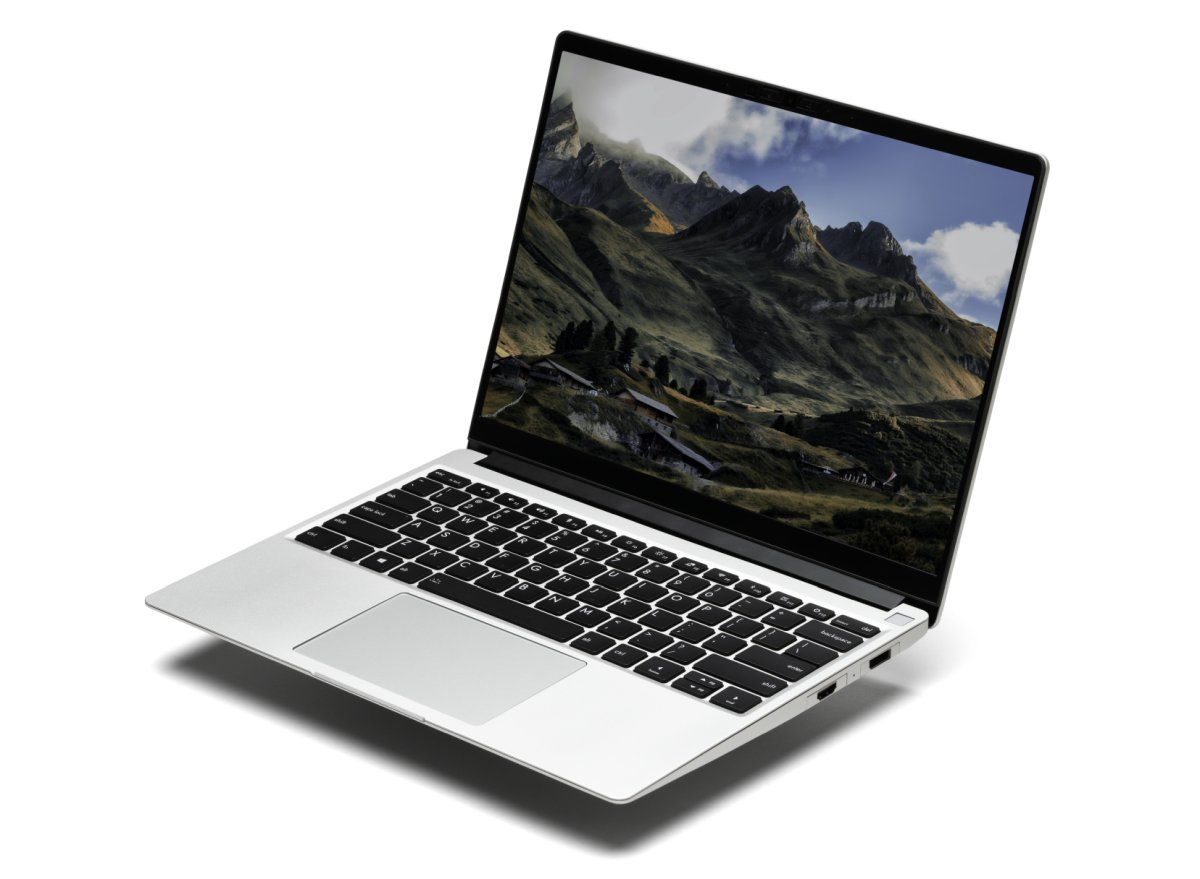
\includegraphics[width=.25\textwidth]{figures/laptop.jpg}};
        \draw[-latex] (llvm.east) -- (framework.west);

        \pause
        \node[below right=-4em and -4.5em of framework] (bug) {
\includegraphics[width=.1\textwidth]{figures/bug.png}};
        \node[above right=-2em and -2em of framework] (snail) {
\includegraphics[width=.1\textwidth]{figures/snail.png}};

        \pause
        \node[above=1em of openssl] (tux){
\includegraphics[width=.15\textwidth]{figures/tux.png}};
        \draw[-latex] (tux.east) -- ++ (1.5,-1);

        \node[below=1em of openssl] (opencv){
\includegraphics[width=.15\textwidth]{figures/opencv.jpg}};
        \draw[-latex] (opencv.east) -- ++ (1.5,+1);

        \pause
        \node[above=1em of framework] (phone){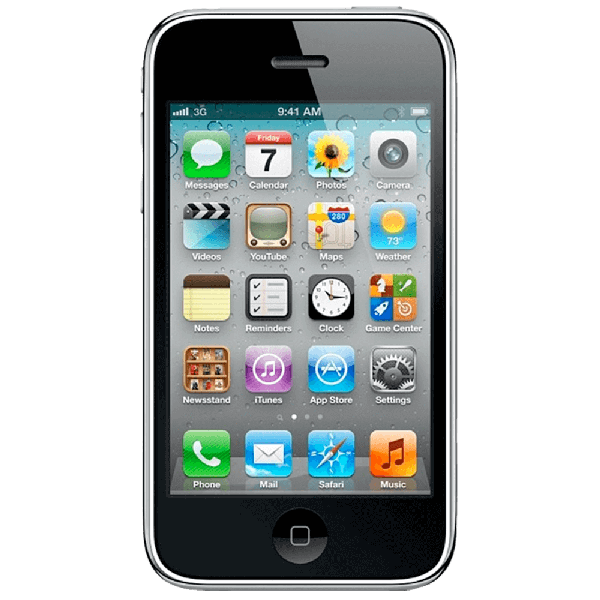
\includegraphics[width=.15\textwidth]{figures/phone.png}};
        \draw[-latex] (llvm.north east) -- (phone.west);

        \node[below=.1em of framework] (bulb){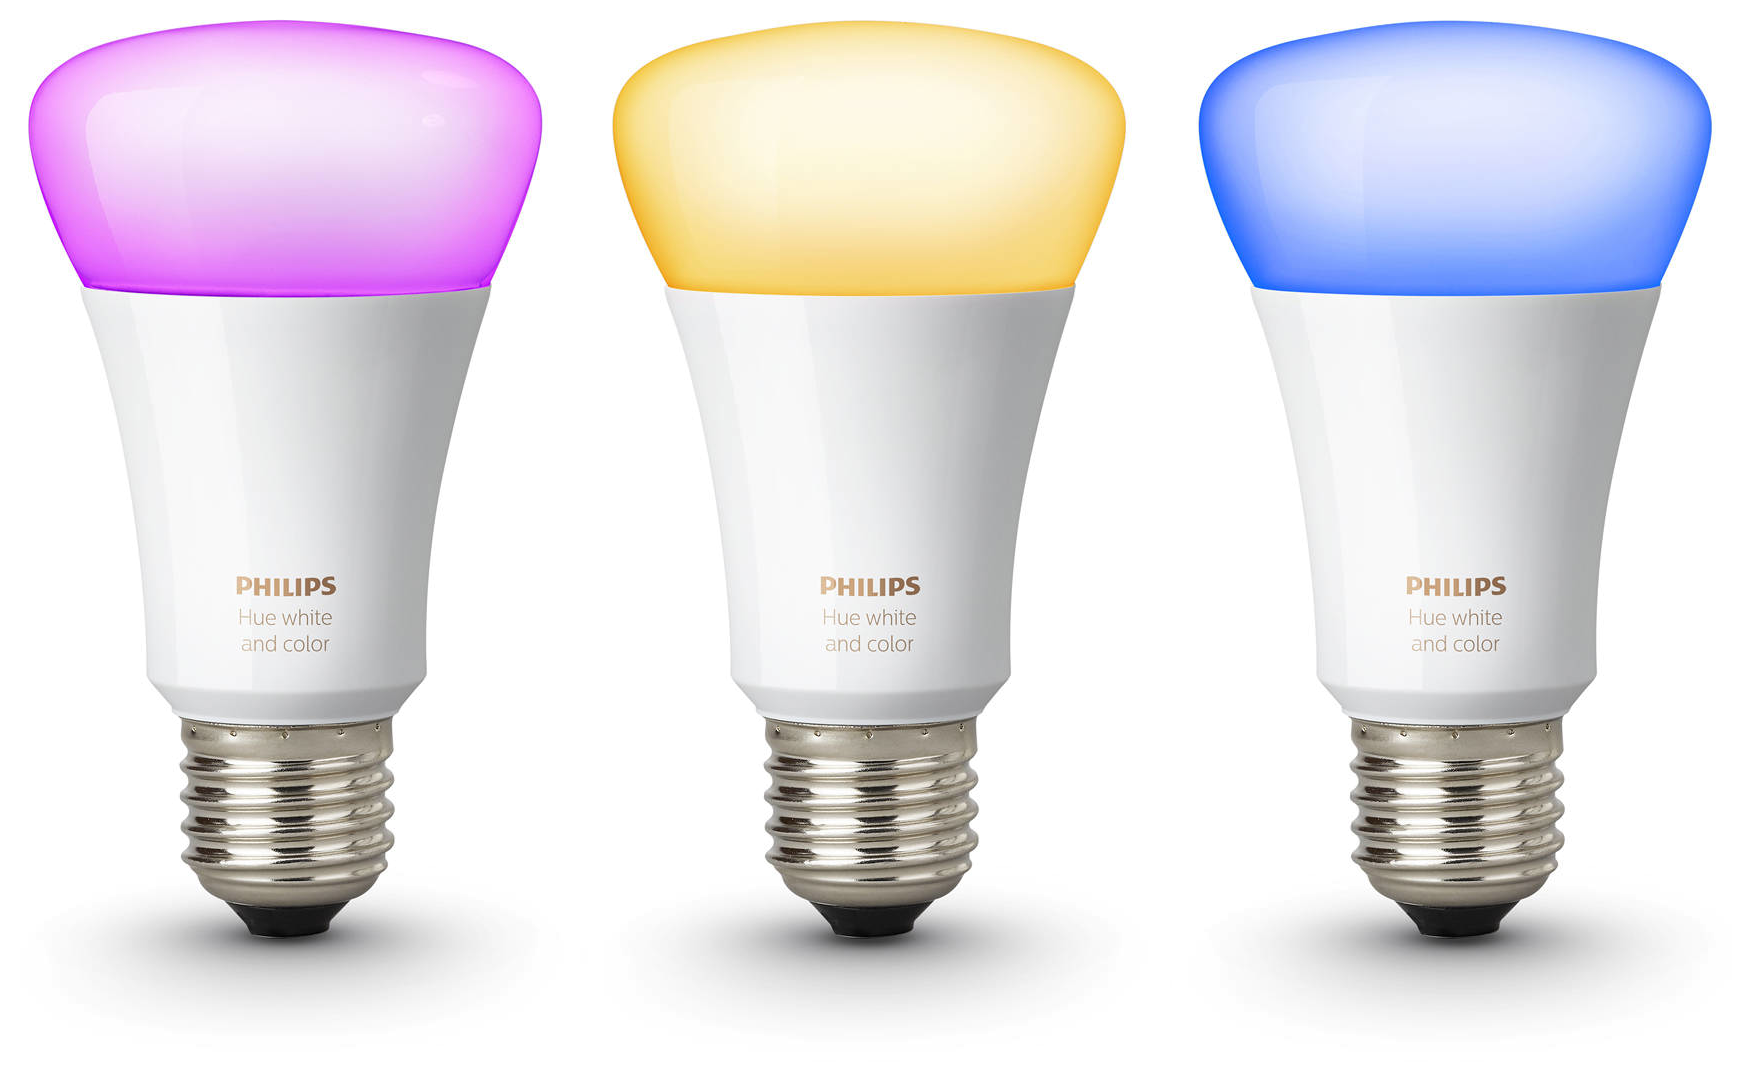
\includegraphics[width=.15\textwidth]{figures/bulb.png}};
        \draw[-latex] (llvm.south east) -- (bulb.west);
    \onslide<1-> %% workaround to have the footline
    \end{tikzpicture}



\end{frame}

\subsection{Code}
\begin{frame}
    \frametitle{\insertsubsection}
    \centering
        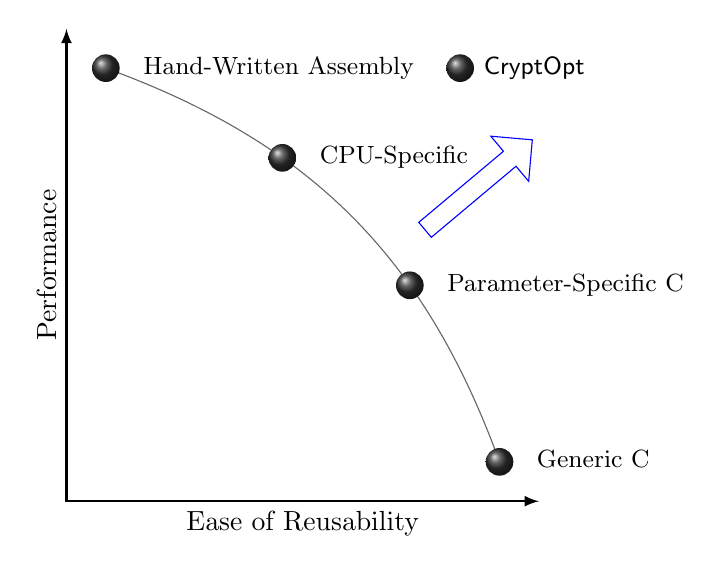
\begin{tikzpicture}[anchor=mid west, mark size=.5em, ball color=black!80]

%
        \pause
        \draw [latex-latex,thick] (0,6)
            -- (0,0) node[rotate=90, midway, above, align=center] {Performance}
            -- (6,0) node[           midway, below, align=center] {Ease of Reusability};

        \draw [draw=black!60] (0.5,5.5) to[out=-20, in=110]
            coordinate[pos=0] (p-4)
            coordinate[pos=1/3] (p-3)
            coordinate[pos=2/3] (p-2)
            coordinate[pos=1] (p-1)
            (5.5,0.5);


        \pause
        \draw[mark options={fill=red}] plot[mark=ball, onslide=<7->{ball color=red!80}    ] coordinates {(p-1)} node[xshift=1em] {\small Generic C};
        \pause
        \draw[mark options={fill=red}] plot[mark=ball, onslide=<7->{ball color=red!80}    ] coordinates {(p-2)} node[xshift=1em] {\small Parameter-Specific C};
        \pause
        \draw[mark options={fill=red}] plot[mark=ball, onslide=<7->{ball color=red!80}    ] coordinates {(p-3)} node[xshift=1em] {\small CPU-Specific};
        \pause
        \draw[mark options={fill=red}] plot[mark=ball, onslide=<7->{ball color=green!80}  ] coordinates {(p-4)} node[xshift=1em] {\small Hand-Written Assembly};

        \pause
        \pause
        \node [single arrow, rotate=40, draw=blue] at (4.5,3.5) {\quad\quad\quad\quad\quad};
        \pause
        \draw[mark options={fill=red}] plot[mark=ball, onslide=<7->{ball color=green!80}  ] coordinates {(5,5.5)} node[xshift=.5em] {\small \cryptopt};

        \onslide<1-> %% workaround to have the footline
    \end{tikzpicture}


\end{frame}

\section{Method}
\subsection{Idea}
\begin{frame}
    \centering
    \frametitle{\insertsubsection}
    \begin{itemize}
        \item Observations:
        \item[1.] Compilers are general-purpose.
        \item<2->[2.] Some code is ``\only<2>{special}\only<3->{\sout{special} \alert<3>{simpler}}''\only<3->{$(X \boldsymbol{+} Y) \boldsymbol{\cdot} Z \boldsymbol{+}Z^2$}.
    \end{itemize}

    \vspace{.5em}
    \onslide<4->{
        \begin{center}
            \emph{(How) can we exploit this?}
        \end{center}
    }
    \vspace{.5em}
    \onslide<5->{
        \begin{itemize}
            \item So\dots
            \item[1.] \sout{Compiling to} $\rightarrow$ \alert<5>{search for} a fast implementation.
            \item<6->[2.] Prove it \alert{correct}.
        \end{itemize}
    }
\end{frame}

\subsection{Search for Fast Implementation}
\begin{frame}[t]{}
    \centering
    \frametitle{\insertsubsection}
    \begin{columns}
        \column{.5\textwidth}
        \centering
        \tikzset{every picture/.style={line width=0.75pt}} %set default line width to 0.75pt        
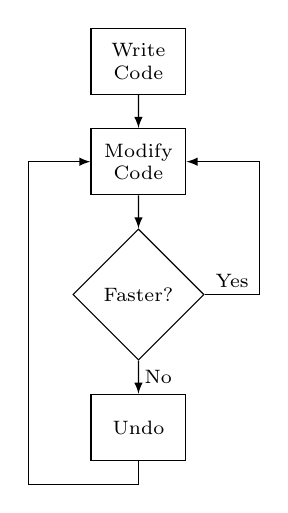
\begin{tikzpicture}[-latex, yscale=.7,xscale=.7]
    \scriptsize
    \tikzstyle{codeblock} = [draw=black, inner sep=.4em, text width=3.5em, minimum height=3em, align=center];

    \pause
    \node[codeblock] (in) at (7,7) {Write Code};

    \pause
    \node[codeblock] (code) [below=1.5em of in] {Modify Code};
    \draw[-latex] (in.south) -- (code.north){};

    \pause
    \node[diamond, draw, below=1.5em of code, text width=4em, align=center] (worse) {Faster?};
    \draw[-latex] (code.south) -- (worse.north){};

    \pause
    \draw[-latex] (worse.east) -- ++(1,0) node[yshift=.6em,midway] {Yes} |- (code.east){};

    \pause
    \node[codeblock] (revert) [below=1.5em of worse] {Undo};
    \draw[-latex] (worse.south) --  node[xshift=0.9em] {No}  (revert.north){};
    \draw[-latex] (revert.south) |- ++(-2,-1.5em) |-  (code.west){};

    \onslide<1-> %% workaround to have the footline
\end{tikzpicture}


        \column{.45\textwidth}
        \onslide<7->{\LARGE ``Random Local Search''}
    \end{columns}
\end{frame}

\newcommand{\cnothing}{c_{\scaleto{\varnothing}{4pt}}}
\newcommand{\ali}[2]{\makebox[#1][r]{#2}}
\subsection{Example}
\begin{frame}[t]{}
    \frametitle{\insertsubsection: $\alert<5>{(X \boldsymbol{+} Y)} \alert<6>{\boldsymbol{\cdot} Z} \alert<8>{\boldsymbol{+}} \alert<7>{Z^2}$}
    \centering

    \vspace{-1em}
    \begin{tikzpicture}[-latex, yscale=.7,xscale=.5, line width=.75pt]
    \scriptsize
    \pause
    \tikzstyle{codeblock} = [draw=black, inner sep=.4em, text width=3.5em, minimum height=3em, align=center];
    \tikzstyle{instr} = [rounded rectangle, draw=black, fill=white, minimum width=1cm, xshift=-.3cm,yshift=-.2cm];
    \tikzstyle{ordermut} = [very thick, dashed, stealth-stealth, red];
    \tikzstyle{highlight} = [fill=red!30];


    \node[codeblock, onslide={<3-12>       {highlight}}] (in) at (7,7)              {Write Code};
    \node[codeblock, onslide={<13-17,20-22>{highlight}}] (code) [below=1.5em of in] {Modify Code};

    \draw[-latex] (in.south) -- (code.north){};
    \only<14->   \node[above right=-.3 and .9 of code.north east, onslide=<15-17>{highlight}, text width=4.4em, align=center] {Instr. scheduling};
    \only<14->   \node[below right=-.3 and .9 of code.south east, onslide=<20-22>{highlight}, text width=4.4em, align=center] {Instr. selection};

    \node[diamond, draw, below=1.5em of code, text width=4em, align=center, onslide={<18,23>{highlight}}] (worse) {Faster?};
    \draw[-latex] (code.south) -- (worse.north){};

    \draw[-latex, temporal=<19>{}{red}{}] (worse.east) -- ++(1,0) node[yshift=.6em,midway] {Yes} |- (code.east){};

    \node[codeblock] (revert) [below=1.5em of worse] {Undo};
    \draw[-latex] (worse.south) --  node[xshift=0.9em] {No}  (revert.north){};
    \draw[-latex] (revert.south) |- ++(-2,-1.5em) |-  (code.west){};


    \pause
    \tikzstyle{operation} = [rounded rectangle, draw=black, minimum width=1cm];
    \tikzstyle{input} = [rounded rectangle, draw=black, fill=white, minimum width=.5cm];
    \tikzstyle{code}  = [text width=4cm, align=left];
    \tikzstyle{ar}    = [-latex, lightgray];

    \pause
    \node [input                ] (Y) at (15,8) {$Y$};
    \node [input, left =4em of Y] (X)           {$X$};
    \node [input, right=4em of Y] (Z)           {$Z$};

    \pause
    \node [operation, \colA, onslide=<21>{highlight}] (A1) at (15, 6) {$\fadd$};
    \draw[ar] (X.south)     -- (A1.north west);
    \draw[ar] (Y.south)     -- (A1.north);

    \pause
    \node [operation, below=4em of A1,  \colB, onslide=<17->{below=9em of A1}] (M1)           {$\fmul$};
    \draw[ar, bend right] (A1.south west)  to node[very near start, xshift=-.2cm] {} (M1.north west);
    \draw[ar] (Z.south)     -- (M1.north east);

    \pause
    \node [operation, below=9em of A1,  \colC, onslide=<17->{below=4em of A1}] (M2)           {$\fmul$};
    \draw[ar] (Z.south) -- (M2.north);
    \draw[ar] (Z.south) -- (M2.north east);

    \pause
    \node [operation, below=14em of A1, \colE] (A2)           {$\fadd$};
    \draw[ar, bend right] (M1.south west)  to node[very near start, xshift=-.2cm] {} (A2.north west);
    \draw[ar, bend right] (M2.south west)  to node[very near start, xshift=-.2cm] {} (A2.north west);


    \pause
    \node [instr, right of=A1, onslide=<21>{highlight}] (iA1) {\only<-21>{\instr{adcx}}\only<22->{\instr{add}}};
    \node [instr, right of=M2] (iM2) {\instr{mulx}};
    \node [instr, right of=M1] (iM1) {\instr{mulx}};
    \node [instr, right of=A2] (iA2) {\instr{add}};

    \pause
    \node [code,        right=  6em of A1] (i1)  {\texttt{mov  rax, [X]}};
    \node [code,        below=.05em of i1] (i2)  {\only<-21>{\texttt{clc          }}\only<22->{\sout{\color{black!60}{\texttt{clc         }}}}};
    \node [code, \colA, below=.05em of i2] (i3)  {\only<-21>{\texttt{adcx rax, [Y]}}\only<22->{\texttt                       {add $\ \,$rax, [Y]}  }};

    \pause
    \node [code,        right=  6em of M1] (i4)  {\textcolor<17->{white}{\texttt{mov  rdx, [Z]}}};
    \node [code, \colB, below=.05em of i4] (i5)  {\texttt{mulx r8, r9, rax}};

    \pause
    \node [code,        right=  6em of M2] (i6)  {\only<17->{\texttt{mov  rdx, [Z]}}};
    \node [code, \colC, below=.05em of i6] (i7)  {\texttt{mulx r10, r11, [Z]}};

    \node [code, \colE, right=  6em of A2] (i8)  {\texttt{add  r11, r9}};
    \node [code,        below=.05em of i8] (i9)  {\texttt{mov  [out], r11}};

    \pause
    \only<16> \draw [ordermut, bend right] (M1.south) to node[midway, xshift=-.3cm] {\quad} (M2.north);


    \onslide<1-> %% workaround to have the footline
\end{tikzpicture}

\end{frame}

\begin{frame}[c]{}
    \frametitle{Performance}
    \centering
    \include{figures/10710Urun1}

\end{frame}

\section{\fiat}
\subsection{Performance}
\begin{frame}[c]{}
    \frametitle{\insertsection}
    \centering
    \vspace{-1em}
    
\tikzset{every picture/.style={line width=0.75pt}} %set default line width to 0.75pt        
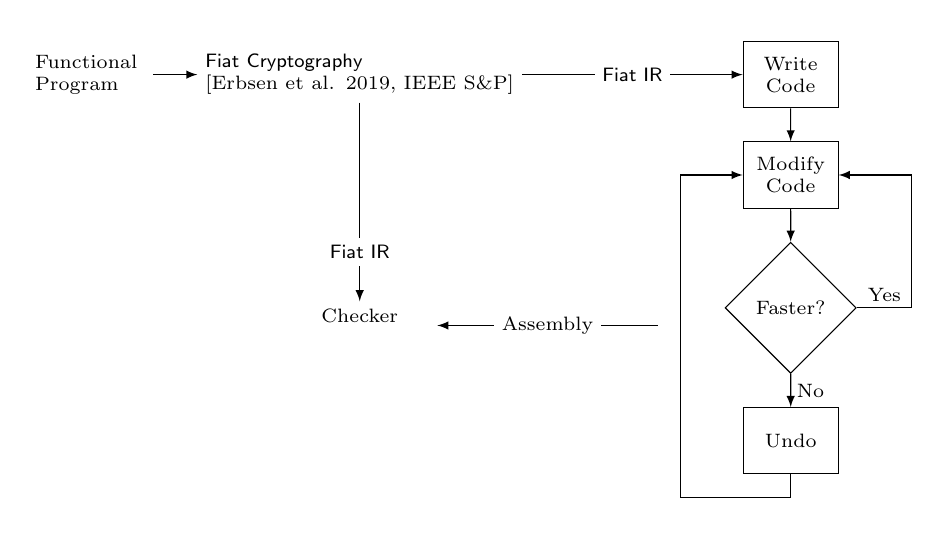
\begin{tikzpicture}[-latex, yscale=.7,xscale=.7]
    \scriptsize
    \tikzstyle{codeblock} = [draw=black, inner sep=.4em, text width=3.5em, minimum height=3em, align=center];


    \node[text width=14em] (fiat) at (0,0) {\fiat\newline [Erbsen et al. 2019, IEEE S\&P]};
    \pause
    \node[text width=5em] (input) [left=2em of fiat] {Functional Program};
    \draw[-latex] (input.east) -- (fiat.west);

    \pause

    \node[codeblock, right=10em of fiat] (in)  {Write Code};

    % Code
    \node[codeblock] (code) [below=1.5em of in] {Modify Code};
    \draw[-latex] (in.south) -- (code.north){};

    \node[diamond, draw, below=1.5em of code, text width=4em, align=center] (worse) {Faster?};
    \draw[-latex] (code.south) -- (worse.north){};
    
    \draw[-latex] (worse.east) -- ++(1,0) node[yshift=.6em,midway] {Yes} |- (code.east){};

    \node[codeblock] (revert) [below=1.5em of worse] {Undo};
    \draw[-latex] (worse.south) --  node[xshift=0.9em] {No}  (revert.north){};
    \draw[-latex] (revert.south) |- ++(-2,-1.5em) |-  (code.west){};

    \node[rectangle,inner ysep=11em, inner xsep=2em, below=-5pt of in.north ] (co) {\quad\quad\quad\quad\quad\quad\quad\quad\quad};

    \pause
    \draw[-latex] (fiat.east) -- node[fill=white, midway]{\fiatir} (in.west);

    \pause
    \draw[-latex] (co.west)+(0,-1) -- node[fill=white, midway]{Assembly} ++(-4,-1); %fiat2.south);

    \pause
    \node [anchor=east, below=9em of fiat](fiat2)   {Checker};
    \draw[-latex] (fiat.south) -- node[fill=white,near end]{\fiatir} (fiat2.north);
    % \pause

    \tikzset{decoration={snake,amplitude=.4mm,segment length=2mm, post length=0mm,pre length=0mm}}
    % \pause

    \onslide<1-> %% workaround to have the footline


\end{tikzpicture}



\end{frame}

\begin{frame}[c]{}
    \centering
    \frametitle{\insertsubsection: Field Arithmetic}

    Geometric Mean (10 $\mu$-Architectures)\\
    \newcommand{\resavgwidth}{2em}
\begin{tabular}{@{}lm{\resavgwidth}m{\resavgwidth}cm{\resavgwidth}m{\resavgwidth}}
    \toprule
                &                                                                    \multicolumn{2}{c}{Multiply}                           &  &                                                         \multicolumn{2}{c}{Square}\\
                                                                                             \cmidrule{2-3}                                                                                                        \cmidrule{5-6} 
    Curve       &                                                    Clang    &                                                     GCC     &  &                                                  Clang      &                                                     GCC \\
    \midrule
    Curve25519  & \only<2->{ \cellcolor{     blue!100}\color{white}{$1.19$} } & \only<2->{ \cellcolor{     blue!100}\color{white}{$1.14$} } &  & \only<2->{ \cellcolor{     blue!100}\color{white}{$1.14$} } & \only<2->{ \cellcolor{     blue!100}\color{white}{$1.18$}} \\
    P-224       & \only<2->{ \cellcolor{     blue!100}\color{white}{$1.31$} } & \only<2->{ \cellcolor{     blue!100}\color{white}{$1.87$} } &  & \only<2->{ \cellcolor{     blue!100}\color{white}{$1.24$} } & \only<2->{ \cellcolor{     blue!100}\color{white}{$1.84$}} \\
    P-256       & \only<2->{ \cellcolor{     blue!100}\color{white}{$1.27$} } & \only<2->{ \cellcolor{     blue!100}\color{white}{$1.79$} } &  & \only<2->{ \cellcolor{     blue!100}\color{white}{$1.30$} } & \only<2->{ \cellcolor{     blue!100}\color{white}{$1.85$}} \\
    P-384       & \only<2->{ \cellcolor{     blue!100}\color{white}{$1.12$} } & \only<2->{ \cellcolor{     blue!100}\color{white}{$1.66$} } &  & \only<2->{ \cellcolor{     blue!76 }\color{white}{$1.08$} } & \only<2->{ \cellcolor{     blue!100}\color{white}{$1.60$}} \\
    SIKEp434    & \only<2->{ \cellcolor{     blue!100}\color{white}{$1.30$} } & \only<2->{ \cellcolor{     blue!100}\color{white}{$1.70$} } &  & \only<2->{ \cellcolor{     blue!100}\color{white}{$1.29$} } & \only<2->{ \cellcolor{     blue!100}\color{white}{$1.83$}} \\
    Curve448    & \only<2->{ \cellcolor{     blue!22 }\color{black}{$1.02$} } & \only<2->{ \cellcolor{   orange!52 }\color{black}{$0.95$} } &  & \only<2->{ \cellcolor{   orange!4  }\color{black}{$1.00$} } & \only<2->{ \cellcolor{   orange!8  }\color{black}{$0.99$}} \\
    P-521       & \only<2->{ \cellcolor{     blue!100}\color{white}{$1.20$} } & \only<2->{ \cellcolor{     blue!58 }\color{white}{$1.06$} } &  & \only<2->{ \cellcolor{     blue!100}\color{white}{$1.25$} } & \only<2->{ \cellcolor{     blue!95 }\color{white}{$1.11$}} \\
    Poly1305    & \only<2->{ \cellcolor{     blue!94 }\color{white}{$1.10$} } & \only<2->{ \cellcolor{     blue!100}\color{white}{$1.15$} } &  & \only<2->{ \cellcolor{     blue!79 }\color{white}{$1.09$} } & \only<2->{ \cellcolor{     blue!100}\color{white}{$1.16$}} \\
    secp256k1   & \only<2->{ \cellcolor{     blue!100}\color{white}{$1.34$} } & \only<2->{ \cellcolor{     blue!100}\color{white}{$1.73$} } &  & \only<2->{ \cellcolor{     blue!100}\color{white}{$1.32$} } & \only<2->{ \cellcolor{     blue!100}\color{white}{$1.74$}} \\
    \bottomrule
\end{tabular}


\end{frame}

\newcommand{\hil}{\cellcolor{lightgray}}
\begin{frame}[c]{}
    \centering
    \frametitle{\insertsubsection: Scalar Multiplication}
    \vspace{-1em}
    \only<2> {\include{figures/scmul}}
    \only<3> {\include{figures/scmul13}}

\end{frame}

\subsection{Correctness}
\begin{frame}[c]{}
    \centering
    \frametitle{\insertsubsection}

    
\tikzset{every picture/.style={line width=0.75pt}} %set default line width to 0.75pt        
\begin{tikzpicture}[-latex, yscale=.7,xscale=.7]
    \scriptsize
    \tikzstyle{codeblock} = [draw=black, inner sep=.4em, text width=3.5em, minimum height=3em, align=center];

    \node[text width=5em] (input) [left=2em of fiat] {Functional Program};
    \draw[-latex] (input.east) -- (fiat.west);

    \node[text width=14em] (fiat) at (0,0) {\fiat\newline [Erbsen et al. 2019, IEEE S\&P]};

    \node[codeblock, right=10em of fiat] (in)  {Write Code};

    % Code
    \node[codeblock] (code) [below=1.5em of in] {Modify Code};
    \draw[-latex] (in.south) -- (code.north){};

    \node[diamond, draw, below=1.5em of code, text width=4em, align=center] (worse) {Faster?};
    \draw[-latex] (code.south) -- (worse.north){};
    
    \draw[-latex] (worse.east) -- ++(1,0) node[yshift=.6em,midway] {Yes} |- (code.east){};

    \node[codeblock] (revert) [below=1.5em of worse] {Undo};
    \draw[-latex] (worse.south) --  node[xshift=0.9em] {No}  (revert.north){};
    \draw[-latex] (revert.south) |- ++(-2,-1.5em) |-  (code.west){};

    \node[rectangle,  inner ysep=11em, inner xsep=2em, below=-5pt of in.north ] (co) {\quad\quad\quad\quad\quad\quad\quad\quad\quad};

    \draw[-latex] (fiat.east) -- node[fill=white, midway]{\fiatir} (in.west);

    \draw[-latex] (co.west)+(0,-1) -- node[fill=white,midway]{Assembly} ++(-4,-1); %fiat2.south);
    \pause
    \node [anchor=east, below=9em of fiat](fiat2)   {Checker};
    \draw[-latex] (fiat.south) -- node[fill=white,near end]{\fiatir} (fiat2.north);
    \pause

    \tikzset{decoration={snake,amplitude=.4mm,segment length=2mm, post length=0mm,pre length=0mm}}
    \draw[decorate,-] (fiat2.south west) -- ++(0,-2);
    \pause
    \draw[decorate,-] (fiat2.south east) -- ++(0,-2);
    \pause
    \node[below=1.2 of fiat2, text width=3em, align=center](equal)  {$\stackrel{?}{=}$};



    \onslide<1-> %% workaround to have the footline


\end{tikzpicture}


\end{frame}



\section{Summary}
\subsection{Summary}
\begin{frame}[c]{}
    \centering
    \frametitle{\insertsubsection}

    \pause
    \begin{columns}
        \column{0.6\textwidth}
        \begin{itemize}
            \item Compilation of cryptographic code \\$\implies$ Search \pause
            \item Random Local Search + Runtime \pause %to find the best implementation code
                % \item Exploit Hardware Properties \pause %Thereby exploit hardware uncertainties (randomly turn those setscrews)\\
            \item \alert<4-5>{Proven-correct} assembly for field arithmetic by \fiat \pause
            with \alert<5>{on-par performance} to hand-optimized assembly. \pause
            \item \alert<6>{Curve25519} assembly in \alert<6>{BoringSSL}.\\
                  \alert<6>{PR \#1329} at \alert<6>{bitcoin-core/secp256k1}.
        \end{itemize}

        \column{0.29\textwidth}
        \centering

        \pause
        GitHub Project
        
\includegraphics[width=10em]{qr.png}
    \end{columns}
    \vskip.5em
    \centerline{\texttt{https://0xade1a1de.github.io/CryptOpt}}


\end{frame}

\appendix

\section{Extras}

\subsection{Bet and Run}
\begin{frame}[c]{}
    \centering
    \frametitle{\insertsubsection}
    \include{figures/10710U}
\end{frame}

\end{document}
